23. $y=\cfrac{\sqrt{(x+1)^2-4x}}{x^2-x}=\cfrac{\sqrt{(x-1)^2}}{x(x-1)}=\cfrac{|x-1|}{x(x-1)}=\begin{cases}\cfrac{1}{x},\ x>1,\\ -\cfrac{1}{x},\ x<1\end{cases}.$
$$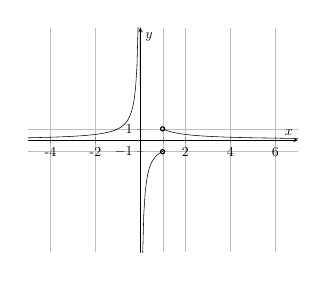
\begin{tikzpicture}[scale=0.5]
\begin{axis}[
    axis lines = middle,
    grid=major,
    legend pos={south west},
    xlabel = {$x$},
    %xlabel style={below right},
    ylabel = {$y$},
    ymin=-10,
    ymax=10,
    xtick={-4, -2,1,2,4,6},
    xticklabels={-4, -2,$ $,2, 4,6},
    ytick={1,-1},
    %yticklabels={-5,-4,$ $,$-\frac{3}{2}$,6},
                  ]
	\addplot[domain=-5:1, samples=100, color=black] {-1/x};
    \addplot[domain=1:7, samples=100, color=black] {1/x};
	%\addlegendentry{$\text{Рис. 1}$};
\end{axis}
\draw (3.42,2.55) circle (1.5pt);
\draw (3.42,3.13) circle (1.5pt);
%\draw (3.7,3.05) circle (2pt);
\end{tikzpicture}$$
